% draft会跳过文档中的所有图片。正式导出时需要删掉draft参数。
\documentclass[12pt, a4paper, oneside]{ctexart}

\usepackage{amsmath}
\usepackage{amssymb}
\usepackage{amsopn}
\usepackage{bm}
\usepackage{graphicx}
\usepackage{mathrsfs}
\usepackage{geometry}
\usepackage{framed}
\usepackage{color}
\usepackage{caption}
\usepackage{listings}
\usepackage{fancyhdr}
\usepackage{booktabs}
\usepackage{makecell}
\usepackage{indentfirst}
\usepackage{authblk}
\usepackage{multicol}
% \usepackage{draftwatermark}       % 需要应用水印时取消注释
\usepackage{enumitem}
\usepackage[hidelinks]{hyperref}
\usepackage{tikz}
\usepackage{ulem}
\usetikzlibrary{positioning, shapes.geometric}

% 分栏线宽
\columnseprule=0.4pt

% 定制第二级无序列表的点样式
\setlist[itemize,2]{label=$\diamond$}

% 页边距
\geometry{a4paper, scale=0.8}

\pagestyle{fancy}

% 调整页眉高度,用于去除警告
\setlength{\headheight}{25pt}

\fancyhf{}      % 清空页眉页脚设置
\fancyhead[L] {
    % 工大计算机系logo
    
\includegraphics[height=7mm]{./images/logo1.jpg}
}
\fancyhead[C]{《数据结构》复习}
\fancyhead[R]{\leftmark}    % 右侧页眉:当前章标题

% 页脚居中放置页码
\fancyfoot[C]{\thepage}

% 设置章节标题自动编号的格式
\ctexset{
  section/number=\chinese{section},
%   subsection/name={,},
%   subsection/number=\chinese{subsection}
}

% 行距。ctexart默认值为1.3
\linespread{1.2}

\lstset{
  language=c,
  basicstyle=\ttfamily,
  frame=single,
  numbers=left
}

% \SetWatermarkText{Eslzzyl整理}            % 设置水印内容
% \SetWatermarkLightness{0.9}             % 设置水印透明度 0-1
% \SetWatermarkScale{0.8}                   % 设置水印大小 0-1

\renewcommand{\headrulewidth}{1pt}  %页眉线宽,设为0可以去页眉线
\renewcommand{\footrulewidth}{1pt}  %脚注线的宽度

\definecolor{shadecolor}{RGB}{241, 241, 255}

\title{
    
\includegraphics[width=0.3\textwidth]{images/hfut-badge.pdf}
    
    \vspace{20pt}
    《数据结构》总复习
}
\author{Eslzzyl}
\date{\today}

\newcounter{problemname}
\newenvironment{problem}{\begin{shaded}\stepcounter{problemname}\par\noindent\textbf{例题\arabic{problemname}. }}{\end{shaded}\par}
\newenvironment{solution}{\begin{shaded}\par\noindent\textbf{解答:}}{\end{shaded}\par}
% \newenvironment{solution}{\par\noindent\textbf{答案. }}{\par}
% \newenvironment{note}{\par\noindent\textbf{例题\arabic{problemname}的注记. }}{\\\par}
\newenvironment{note}{\par\noindent\textbf{注记. }}{\par}

\begin{document}

\maketitle
\newpage
\tableofcontents
\vspace{20pt}
% 如果在目录处有备注,可以写在这里。

\newpage

\section{绪论}

\subsection{数据结构的基本概念}

\subsubsection{基本概念和术语}

\begin{itemize}
  \item {\bf 数据},是信息的载体,是计算机程序加工的原料。
  \item {\bf 数据元素},是数据的基本单位,如一个学生记录。可由若干个数据项组成,如包含学号、姓名、性别等数据项。
  \item {\bf 数据对象},是具有\textbf{相同性质}的数据元素的集合。
  \item {\bf 数据类型},是一个值的集合和定义在此集合上的一组操作的总称。
  \begin{itemize}
    \item 原子类型:不可再分的数据类型。
    \item 结构类型:可以再分的数据类型。
    \item 抽象数据类型
  \end{itemize}
  \item {\bf 数据结构},是相互之间存在一种或多种特定关系的数据元素的集合。数据结构包括三方面内容:
  \begin{itemize}
    \item 逻辑结构,决定算法的设计
    \item 存储结构,又叫映像,决定算法的实现
    \item 数据的运算
  \end{itemize}
\end{itemize}

\subsubsection{数据结构三要素}

\begin{enumerate}
  \item {\bf 数据的逻辑结构}
  
  \begin{figure}[h]
    \centering
    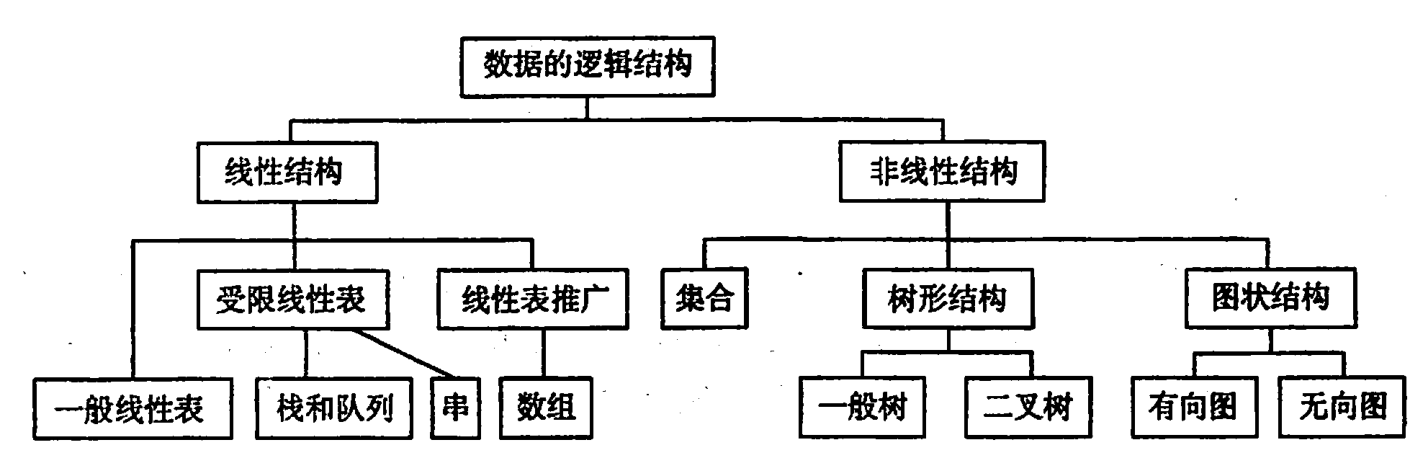
\includegraphics[width=0.7\textwidth]{./images/logical-structure.png}
    \caption{数据的逻辑结构}
    \label{logical-structure}
  \end{figure}
  
  逻辑结构可分为线性结构和非线性结构。见图\ref{logical-structure}。

  \begin{itemize}
    \item {\bf 集合}:结构中的元素之间除了“同属一个集合”之外,没有别的关系。
    \item {\bf 线性结构}:元素之间存在一对一的关系。
    \item {\bf 树形结构}:元素之间存在一对多的关系。
    \item {\bf 图状结构或网状结构}:元素之间存在多对多的关系。
  \end{itemize}

  \item {\bf 数据的存储结构}
  
  存储结构是用计算机语言实现的逻辑结构。
  \begin{itemize}
    \item {\bf 顺序存储}
    \item {\bf 链式存储}
    \item {\bf 索引存储}
    \item {\bf 散列存储}
  \end{itemize}

  \item {\bf 数据的运算}
\end{enumerate}

\subsection{算法和算法评价}

\subsubsection{算法的基本概念}

算法(Algorithm)是对特定问题求解步骤的一种描述。有以下5个重要特性:
\begin{enumerate}
  \item {\bf 有穷性},算法必须在有限个步骤之后结束,且每一步必须消耗有限的时间。
  \item {\bf 确定性},同一个算法对同一个输入必定得出相同的输出。
  \begin{itemize}
    \item 随机类算法不违反确定性,因为计算机是伪随机,对于同一个随机种子,生成的随机数序列总是一致的。
  \end{itemize}
  \item {\bf 可行性}
  \item {\bf 输入},算法有0个或更多个输入。
  \item {\bf 输出},算法有一个或更多个输出。
\end{enumerate}

设计一个好的算法应该考虑:
\begin{itemize}
  \item 正确性
  \item 可读性
  \item 健壮性
  \item 高效率与低存储量需求
\end{itemize}

\subsubsection{算法效率的度量}

\begin{enumerate}
  \item {\bf 时间复杂度}
  
  通常采用算法中基本运算的频度来分析时间复杂度。

  一般总是考虑在最坏情况下的时间复杂度。

  常见的渐进时间复杂度:
  \begin{equation*}
    O(1)<O(\log_2 n)<O(n)<O(n\log_2 n)<O(n^2)<O(n^3)<O(n!)<O(n^n)
  \end{equation*}
  \item {\bf 空间复杂度}
  
  算法\textbf{原地工作}是指算法所需的辅助空间为常量,即$O(1)$。
\end{enumerate}

\section{线性表}

\subsection{线性表的定义和基本操作}

\subsubsection{线性表的定义}

线性表是具有相同数据类型的$n$($n\geq 0$)个数据元素的有限序列,其中$n$为表长。
\begin{equation*}
  L=(a_1,a_2,\cdots,a_i,a_{i+1},\cdots,a_n)
\end{equation*}

线性表的特点:
\begin{itemize}
  \item 表中元素的个数有限。
  \item 元素具有逻辑上的顺序性。
  \item 元素都是数据元素。
  \item 元素的数据类型都相同,占有相同大小的存储空间。
  \item 元素具有抽象性,不关心元素中保存的是什么内容。
\end{itemize}

线性表是逻辑结构,顺序表和链表是物理结构。

\subsubsection{线性表的基本操作}

\begin{itemize}
  \item \verb|InitList(&L)|:初始化表,构造一个空的线性表。
  \item \verb|Length(L)|:返回表的长度
  \item \verb|LocateElem(L, e)|:按值查找
  \item \verb|GetElem(L, i)|,按位置查找
  \item \verb|ListInsert(&L, i, e)|:插入
  \item \verb|ListDelete(&L, i, &e)|:删除
  \item \verb|PrintList(L)|:输出表
  \item \verb|Empty(L)|:判空,空返回\verb|true|
  \item \verb|DestroyList(&L)|:销毁表
\end{itemize}

\subsection{线性表的顺序表示}

注意线性表的下标是从1开始算,数组的下标是从0开始算。

时间复杂度分析(平均):
\begin{itemize}
  \item 随机访问:$O(1)$
  \item 插入:$O(n)$
  \item 删除:$O(n)$
  \item 顺序查找:$O(n)$
\end{itemize}

\subsection{线性表的链式表示}

链表往往引入头结点,有如下好处:
\begin{itemize}
  \item 在链表的第一个位置上的操作和其他位置一致,无需进行特殊处理。
  \item 无论链表是否为空,头指针都指向一个节点,这样空表和非空表的处理得到了统一。
\end{itemize}

建立新链表:
\begin{itemize}
  \item 头插:在头部插入节点,形成的链表的顺序是反的。
  \item 尾插:在尾部插入节点,顺序正常,但需要添加额外的尾指针。
\end{itemize}

时间复杂度分析:
\begin{itemize}
  \item 建立新链表(头插/尾插):$O(n)$
  \item 按序号查找:$O(n)$
  \item 按值查找:$O(n)$
  \item 按值删除:主要耗费在查找上。$O(n)$
  \item 按值插入:同上
  \item 求表长:$O(n)$
\end{itemize}

插入元素时,往往要先找到元素所在的位置,然后执行后插。查找的复杂度是$O(n)$,后插的复杂度仅为$O(1)$。因此:
\begin{itemize}
  \item 当给出插入位置的值时,总复杂度为$O(n)$;
  \item 当给出插入位置的地址时,总复杂度为$O(1)$。
\end{itemize}

有时需要前插,此时要找到目标结点的前面一个节点。对于单链表,必须按照顺序向后查找。此时无论给出的是值还是地址,总复杂度都为$O(n)$;但有一种优化方法:在目标结点的后继插入,然后交换目标结点和新插入结点的值。此时已知地址时,总复杂度为$O(1)$。

类似地,删除结点时,必须得知前驱结点,这样才能正确设置链接关系。但如果直接将后继结点的值赋予待删除结点,然后删除后继结点,这样也能有$O(1)$时间复杂度。

\subsubsection{双链表}

\subsubsection{循环链表}

循环单链表的判空条件不是头结点的指针是否为空,而是它是否等于头指针。

循环单链表少用头指针而多用尾指针。因为尾指针的\verb|next|就是头结点。

\subsubsection{静态链表}

静态链表是用数组实现的链表。不太方便,但是适合没有指针的语言。

\subsubsection{顺序表的链表的比较}

\begin{itemize}
  \item {\bf 存取(读写)方式}
  
  顺序表既能顺序读取,又能随机读取;链表只能顺序读取。

  \item {\bf 逻辑结构与物理结构}
  
  逻辑上都是线性表,但顺序表的结点物理上也是连续的,链表的结点靠指针维持连续性。

  \item {\bf 查找、插入和删除操作}
  \begin{itemize}
    \item 对于按值查找,若表无序,则二者均为$O(n)$;若有序,则顺序表可用二分查找,$O(\log_2 n)$。
    \item 对于按序号查找,顺序表可以随机访问,$O(1)$;链表则为$O(n)$。
  \end{itemize}

  对于插入和删除操作,顺序表的平均复杂度为$O(n)$,链表为$O(1)$。

  \item {\bf 空间分配}
  
  顺序表的分配比较繁琐,链表的分配灵活高效。
\end{itemize}

\section{栈、队列和数组}

本章多为选择题。

\subsection{栈}

\subsubsection{栈的基本概念}

后进先出(LIFO)

$S=(a_1,a_2,a_3,a_4,a_5)$,则$a_1$是栈底,$a_5$是栈顶。

$n$个不同元素进栈,出栈元素共有$\frac{1}{n+1}C_{2n}^n$种不同的排列(卡特兰数,组合数学)。

基本操作:
\begin{itemize}
  \item \verb|InitStack(&S)|:初始化一个空栈。
  \item \verb|StackEmpty(S)|:判断是否为空,空返回\verb|true|。
  \item \verb|Push(&S, x)|:入栈
  \item \verb|Pop(&S, &x)|:出栈
  \item \verb|GetTop(S, &x)|:读栈顶元素
  \item \verb|DestroyStack(&S)|:销毁栈并释放空间。
\end{itemize}

\subsubsection{栈的顺序存储结构}

即用数组实现的栈。需要特别注意入栈时的判满,小心数组越界。

还有一种共享栈,由两个栈共享同一个数组,栈底分布在数组的两端,然后向数组的中间生长。当两个栈顶指针相邻时,判为栈满。

\subsubsection{栈的链式存储结构}

和链表类似。

\subsection{队列}

\subsubsection{队列的基本概念}

先进先出(FIFO)

基本操作:
\begin{itemize}
  \item \verb|IniteQueue(&Q)|:初始化一个空队列。
  \item \verb|QueueEmpty(Q)|:判空,若空返回\verb|true|。
  \item \verb|EnQueue(&Q, x)|:入队
  \item \verb|DeQueue(&Q, &x)|:出队
  \item \verb|GetHead(Q, &x)|:获得队头元素
\end{itemize}

\subsubsection{队列的顺序存储结构}

因队列本身的性质,顺序结构的队列通常设计成循环队列。设置一个队首指针\verb|Q.front|和一个尾后指针\verb|Q.rear|:
\begin{itemize}
  \item 初始时(也是队空条件):\verb|Q.front == Q.rear|
  \item 队首指针进1:\verb|Q.front = (Q.front + 1) % MaxSize|
  \item 队尾指针进1:\verb|Q.rear = (Q.rear + 1) % MaxSize|
  \item 队列长度:\verb|(Q.rear + MaxSize - Q.front) % MaxSize|
  \item 队满:\verb|(Q.rear + 1) % MaxSize == Q.front|
\end{itemize}

\subsubsection{队列的链式存储结构}

是一个带有头指针和尾指针的单链表。两个指针都为空时,表示队列为空。

\subsubsection{双端队列}

王道书写得相当复杂。

双端队列出队时,先进的元素总是排在后出的元素的前面。

受限的双端队列:
\begin{itemize}
  \item 输入受限的双端队列:允许在一端进行插入和删除,但在另一端只允许删除。
  \item 输出受限的双端队列:允许在一端进行插入和删除,但在另一端只允许插入。
\end{itemize}
若进一步限制从某端插入的元素只能在这一端删除,则队列变为两个栈底相邻的栈。

\subsection{栈和队列的应用}

\subsubsection{栈在括号匹配中的应用}

容易

\subsubsection{栈在表达式求值中的应用}

这里只是介绍了栈处理后缀表达式的过程,容易。

\subsubsection{栈在递归中的作用}

没讲什么实质的东西

\subsubsection{队列在层次遍历中的应用}

队列遍历二叉树:
\begin{enumerate}
  \item 根节点入队。
  \item 若队空,结束,否则转3
  \item 队列中的第一个结点出队,并访问之。若其有左孩子,则将左孩子入队;若其有右孩子,则将右孩子入队,然后返回2。
\end{enumerate}

\subsubsection{队列在计算机系统中的应用}

队列可用于解决:
\begin{itemize}
  \item 主机和外设速度不匹配的问题:设置缓冲区队列
  \item 多用户引起的资源竞争问题:设置请求队列
\end{itemize}

\subsection{数组和特殊矩阵}

\subsubsection{数组的定义}

数组是线性表的推广(数组可有多维)。一维数组可视为一个线性表,二维数组可视为其元素也是定长线性表的线性表,依此类推。数组一旦被定义,其长度就固定下来。

\subsubsection{数组的存储结构}

二维数组有按行优先和按列优先。

\subsubsection{特殊矩阵的压缩存储}

特殊矩阵指的是有许多相同的矩阵元素,且分布有一定规律的矩阵,如对称矩阵、上/下三角矩阵、对角矩阵等。

\begin{enumerate}
  \item {\bf 对称矩阵}
  
  对称矩阵只有一半的存储空间是有意义的。因此将其存放在一个一维数组\verb|B[n(n+1)/2]|中,即元素$a_{i,j}$存放在$b_k$中。

  \item {\bf 对角矩阵}
  
  \item {\bf 三对角矩阵}
  
  \item {\bf 稀疏矩阵}
  
  可将非零元素及其所在的行、列构成一个三元组存放起来。这样稀疏矩阵也失去了随机存取特性。
\end{enumerate}

\section{字符串}

本章的重点是模式匹配。

\subsection{字符串的定义和实现}

\subsubsection{字符串的定义}

字符串是由零个或多个字符组成的有限序列:
\begin{equation*}
  S='a_1 a_2 \cdots a_n'\quad (n\geq 0)
\end{equation*}

\subsubsection{字符串的存储结构}

\begin{enumerate}
  \item {\bf 定长顺序存储表示}
  
  规定最大长度,超出长度时直接截断。

  \item {\bf 堆分配存储表示}
  
  动态分配堆内存来存储。

  \item {\bf 块链存储表示}
  
  类似链表,每个结点可以存一个字符,也可以存多个字符,每个结点称为块。最后一个结点占不满时用\verb|#|补上。
\end{enumerate}

\subsubsection{字符串的基本操作}

\begin{itemize}
  \item \verb|StrAssign(&T, chars)|:赋值操作,把字符串\verb|T|赋值为\verb|chars|。
  \item \verb|StrCopy(&T, S)|,复制操作,将\verb|S|复制到\verb|T|。
  \item \verb|StrEmpty(S)|:判空。若为空,返回\verb|true|。
  \item \verb|StrCompare(S, T)|:比较。若\verb|S>T|,则返回值大于0,若等于则返回0,若小于则返回值小于0。
  \item \verb|StrLength(S)|:求长度。
  \item \verb|SubString(&Sub, S, pos, len)|:求子串。通过\verb|Sub|返回\verb|S|的第\verb|pos|个字符起,长度为\verb|len|的字串。
  \item \verb|Concat(&T, S1, S2)|:将\verb|S1|和\verb|S2|拼接,通过\verb|T|返回。
  \item \verb|Index(S, T)|:若\verb|S|中存在\verb|T|,则返回它第一次出现的位置,否则返回0。
  \item \verb||
\end{itemize}

\subsection{字符串的模式匹配}

\subsubsection{简单的模式匹配算法}

\begin{lstlisting}
  int Index(SString S, SString T) {
    int i = 1, j = 1;
    while (i <= S.length && j <= T.length) {
      if (S.ch[i] == T.ch[j]) {
        ++i;
        ++j;
      } else {
        i = i - j + 2;
        j = 1;
      }
    }
    if (j > T.length)
      return i - T.length;
  }
\end{lstlisting}

\subsubsection{KMP算法}

待补

\section{树}

\subsection{树的基本概念}

\subsubsection{树的定义}

树是$n$个结点的有限集。当树不为空时,需要满足:
\begin{enumerate}
  \item 有且仅有一个根节点。
  \item $n>1$时,其余结点可分为$m$个互不相交的有限集$T_1, T_2, \cdots, T_m$,其中每个集合又是一棵树,称为根的子树。
\end{enumerate}

树的定义是递归的。

\begin{itemize}
  \item 除了根节点之外,所有结点有且仅有一个前驱(父节点)。
  \item 所有结点可以有零个或多个后继(子节点)。
\end{itemize}

$n$个结点的树中有$n-1$条边。

\subsubsection{基本术语}

此处只记录一些不太熟悉的。

\begin{itemize}
  \item 一个结点的孩子的数量称为该节点的\textbf{度}。度最大的结点的度称为树的度。
  \item 树的层次从根开始定义,根节点是第一层,然后向下是第二层,以此类推。双亲在同一层的结点互为\textbf{堂兄弟}。
  \item 结点的深度是从根节点开始算的。
  \item 结点的高度是从叶子节点开始算的。
  \item 树的高度(或深度)是树中结点的最大层数。
  \item 树中两个结点之间的路径是由这两个结点之间所经过的结点序列构成的,而路径长度是路径上经过的边的个数。
\end{itemize}

\subsubsection{树的性质}

\begin{itemize}
  \item 树中的结点数等于所有结点的度数之和加1。
  \item 度为$m$的树中第$i$层上至多有$M^{i-1}$个结点。
  \item 高度为$h$的$m$叉树至多有$\frac{m^h-1}{m-1}$个结点。
  \begin{itemize}
    \item $S=m^{h-1}+m^{h-2}+m^{h-3}+\cdots +m+1=\frac{m^h-1}{m-1}$
  \end{itemize}
  \item 具有$n$个结点的$m$叉树的最小高度为$\left\lceil \log_m(n(m-1)+1)\right\rceil $。
\end{itemize}

\subsection{二叉树的概念}

\subsubsection{二叉树的定义及其主要特性}

二叉树的左右子树顺序不能颠倒。

二叉树和度为2的有序树有区别:
\begin{itemize}
  \item 度为2的有序树至少有3个结点,二叉树可以为空,也可以只有根结点。
  \item 度为2的有序树的左右次序是相对于另一个孩子而言的,如果只有一个孩子,那就无需区分左右。二叉树总是要区分左右。
\end{itemize}

一些特殊的二叉树:
\begin{itemize}
  \item {\bf 满二叉树}。高度为$h$,结点数为$2^h-1$的二叉树是满二叉树。满二叉树可以编号,根结点为1,左孩子为2,右孩子为3。这样,对于任意一个结点,它的父节点是$\left\lfloor i/2 \right\rfloor$,左孩子是$2i$,右孩子是$2i+1$。
  \item {\bf 完全二叉树}。
\end{itemize}

\end{document}